\subsection{Biography}
\label{sec:biography}

\begin{wrapfigure}{l}{0.2\textwidth} % "l" for left and "0.25\textwidth" for the width of the wrap figure area
\centering
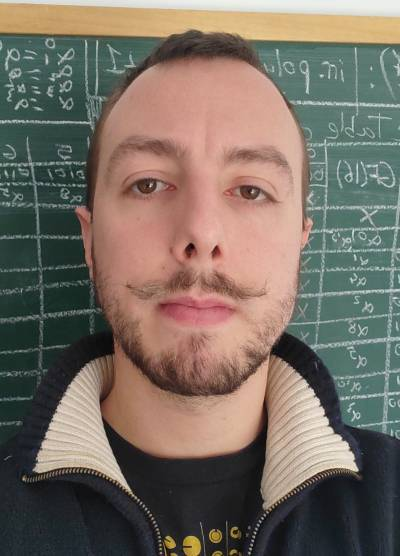
\includegraphics[width=0.18\textwidth]{./figures/louis2.jpg}
\end{wrapfigure}
Louis Ledoux, originating from a comprehensive computer science background in Rennes (Bretagne, France), has transitioned towards a hardware focus. His journey began with a Bachelor's degree, followed by a Master's in Computer Science, culminating in a one-year internship in 2017, where he explored FPGA virtualization in the cloud. Since 2018, Louis has been engaged in a PhD in computer arithmetic at the Universitat Polit\`ecnica de Catalunya and the Barcelona Supercomputing Center, in Barcelona, Spain. His main focus are hardware implementations to address numerical requirements sparsity in HPC workloads. Beyond academia, Louis contributes to the open hardware community, participating in efabless/skywater/Google tapeouts.

%\begin{figure}[H]
%\begin{minipage}[b]{0.1\linewidth}
%\centering
%	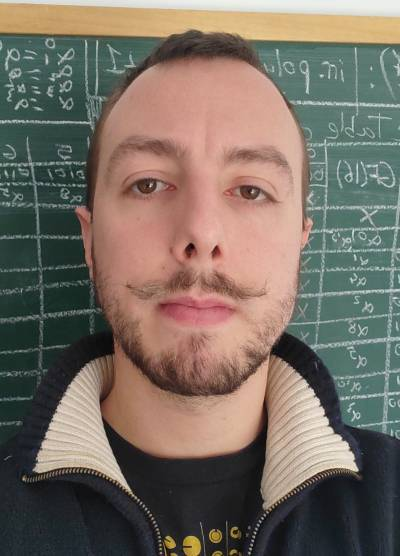
\includegraphics[width=\textwidth]{./figures/louis2.jpg}
%\end{minipage}
%\hspace{0.5cm}
%\begin{minipage}[b]{0.85\linewidth}
%\centering
%Louis Ledoux, originating from a comprehensive computer science background in Rennes (Bretagne, France), has transitioned towards a hardware focus.
%His journey began with a Bachelor's degree, followed by a Master's in Computer Science, culminating in a one-year internship in 2017, where he explored FPGA virtualization in the cloud.
%Since 2018, Louis has been engaged in a PhD in computer arithmetic at the Universitat Polit\`ecnica de Catalunya and Barcelona Supercomputing Center, in Barcelona, Spain.
%His main focus are hardware implementations to address numerical requirements sparsity in HPC workloads.
%Beyond academia, Louis contributes to the open hardware community, participating in efabless/skywater/Google tapeouts.
%\end{minipage}
%\end{figure}
